% 620_abawd_5slides.tex
% Five-slide scaffold on the ABAWD waiver / weighted-set-packing project.
% Meant to be presented alongside the interactive waiver-map artifact
% (6_present/61_waiver_map/611_waiver_map.html), so the slides carry the
% argument and the artifact carries the detail.
%
% Compile from the project root with XeLaTeX (metropolis wants Fira Sans):
%   latexmk -xelatex -cd 6_present/62_abawd_slides/620_abawd_5slides.tex
%
% Convention used throughout: visible text is a minimal skeleton for Joshua
% to fill in; every "% >>" comment is suggested body text, drawn from Julian's
% QE summary slides (qe_project_summary2.pdf pp. 29-36), the paper draft
% (5_write/weighted_set_packingv2.pdf), the rules KB (0_lit/00_abawd_rules),
% and the extraction protocol / progress table. Delete or promote as you like.

\documentclass[aspectratio=169, 11pt]{beamer}

\usetheme{metropolis}
\metroset{
  % block=fill,          % filled block backgrounds (the block+itemize layout reads better)
  sectionpage=none,
  numbering=fraction,
  % progressbar=frametitle
}

\usepackage{amsmath, amssymb}
\usepackage{booktabs}
\usepackage{graphicx}
\usepackage{hyperref}

\graphicspath{{figs/}}

% Tighten the nested itemize inside blocks a little.
\setbeamertemplate{itemize items}[circle]
\setlength{\leftmargini}{1.2em}
\setlength{\leftmarginii}{1.2em}

\newcommand{\Rj}[1]{R^{\mathrm{#1}}}

\title{Can Bureaucrats Solve NP-Complete Problems\\ (and Do They Even Want To)?}
\author{Joshua Levy, Julian Duggan}
\institute{University of Southern California}
\date{\today}

\begin{document}

\maketitle

% =====================================================================
\begin{frame}{Motivation (SNAP)}
  % >> Framing (from Julian's slide 30): ~12% of the US population receives
  % >> SNAP; program is ~0.4% of GDP. Able-Bodied Adults Without Dependents
  % >> (ABAWDs, 18-49/now 18-64) face a 3-months-in-36 time limit unless they
  % >> work/train 20 hrs per week; searching for work is not enough.

  \begin{block}{Supplemental Nutritional Assistance Program}
    \begin{itemize}
      \item SNAP covers $\sim 12\%$ of the population (about $\sim 0.4\%$ of GDP)
      \item 1996: Introduce ``work requirements'' for ``ABAWDs''
      \item ``Areas'' with ``insufficient jobs'' can apply to USDA-FNS for waivers
    \end{itemize}
  \end{block}

  \begin{block}{Why this is a good laboratory}
    \begin{itemize}
      \item What constitutes an ``area'' or ``insufficient jobs'' is ambiguous
      \item 50+ decision makers over $\sim$30 years
    \end{itemize}
  \end{block}
\end{frame}

% =====================================================================
\begin{frame}{A complex regulatory environment}
  % >> Julian's slide 32 states the core rule; the KB (001_abawd_waiver_rules.md)
  % >> has the full two-level structure. Point the audience to the artifact's
  % >> "rules" tab for the effective-dated detail rather than listing it here.

  \begin{block}{Two statutory prongs, several operational routes}
    \begin{itemize}
      \item \textbf{Statutory threshold}
            \begin{itemize}
              \item \textbf{10\% Rule:} area unemployment $>10\%$ (12-mo, 3-mo) self-certifiable (survives the OBBB)
            \end{itemize}
      \item \textbf{``Insufficient jobs''}
            \begin{itemize}
              \item \textbf{LSA:} If DoL assigns this BLS unit (county) to be a ``Labor Surplus Area''
              \item \textbf{EB trigger:} Applies statewide if state is on the BLS ``trigger list'' for extended unemployment benefits
              \item \textbf{20\% Rule:} If the avg. unemployment rate over 24 months in an ``area'' is $20\%$ above the national average in the same 24-month window.
              \item Some federal exemptions (ARRA, FFCRA)
            \end{itemize}
    \end{itemize}
  \end{block}

\end{frame}

% =====================================================================
\begin{frame}{The 20\% rule and room for computational sophistication}
  \begin{block}{State agency's choices}
    \begin{enumerate}
      \item Choice of 24-month data window (starting after Jan of 2/3 FYs prior)
      \item Choice of application date and waiver start date
      \item Choice of (contiguous) LAUS units
      \item Choice of group construction
      \item Choice of BLS data vintage
      \item Rounding rules \ldots
    \end{enumerate}

  \end{block}

\end{frame}

% =====================================================================
\begin{frame}{The math of the weighted set-packing problem}
  % >> Follows Julian's slide 34 and paper Sec. 3. Fixed-window version shown;
  % >> the cross-window version replaces the slack condition with "exists w in
  % >> W(t_app, t_start)". The artifact's set-packing tab has a playable 6x6
  % >> demo that beats greedy -- switch to it here.

  \begin{block}{Primitives (fix a state $s$ and a 24-month window)}
    \begin{itemize}
      \item Counties $i \in I$: labor force $L_i$, unemployed $U_i$, policymaker value $V_i$.
      \item Threshold $\alpha = 1.2\,\tilde{\alpha}$ ($\tilde\alpha$ = national rate); slack $s_i := U_i - \alpha L_i$.
            % >> The slack form is the useful one: a group clears the threshold iff
            % >>   its surpluses cover its deficits, so a small county far above
            % >>   threshold can "carry" a large neighbour just below it (AR FY2008;
            % >>   MT FY2016 bundles where EVERY member is below threshold).
    \end{itemize}
  \end{block}

  \begin{block}{The state's problem}
    \setlength{\abovedisplayskip}{2pt}\setlength{\belowdisplayskip}{4pt}
    \begin{equation*}
      \max_{G \in \mathcal{P}(\mathcal{P}(I))} \; \sum_{g \in G} \sum_{i \in g} V_i
      \quad \text{s.t.} \quad
      g \text{ contiguous}, \;\;
      g \cap g' = \varnothing, \;\;
      \textstyle\sum_{i \in g} s_i \ge 0
      \qquad \forall\, g \neq g' \in G
    \end{equation*}
    % >> Cross-window version (paper eq. 6): replace the slack condition with
    % >>   "exists w in W(t_app, t_start) with sum_i s_iw >= 0" -- the window
    % >>   choice is itself part of the state's problem.
    % \begin{itemize}
    % \item Enumerate admissible groups $C = \{g_1,\dots,g_K\}$, weights $W_k = \sum_{i \in g_k} V_i$; then
    % $\max_{y \in \{0,1\}^K} \sum_k W_k y_k$ s.t. $\sum_{k:\, i \in g_k} y_k \le 1$ $\forall i$.
    % >> This is weighted set packing: NP-complete in general, but instances
    % >>   here are small enough for Gurobi (Julian) / the artifact's
    % >>   enumerative solver (contiguous groups up to size 6).
    % >> Greedy (commit highest-weight disjoint group, repeat) is the natural
    % >>   heuristic and carries no guarantee -- one candidate "capacity"
    % >>   account of sub-optimal allocations.
    % \end{itemize}
  \end{block}
\end{frame}

% =====================================================================
\begin{frame}{Notions of optimality -- Preferences?}
  % >> Paper Sec. 4.1-4.2 and Julian's slide 35. The point of this slide is
  % >> that "optimal" is only defined relative to a valuation scheme, and the
  % >> scheme is itself the object of inference.

  \begin{block}{Valuation schemes $V^j$ (increasing sophistication)}
    \begin{itemize}
      \item $\Rj{N}$: $V_i = 1$ \quad $\Rj{pop}$: $V_i = $ population \quad $\Rj{SNAP}$: $V_i = $ SNAP recipients
            % >> V^N: maximize the number of waived counties.
            % >> V^pop: maximize population living in waived areas.
            % >> V^SNAP: maximize SNAP recipients (Census/ACS) in waived areas.
            % >> Ideal target (paper fn. 24): V_i^tau = Y_i(1) - Y_i(0), the
            % >>   treatment effect on ABAWD enrollment; proxied by ABAWD counts
            % >>   at application date (CPS), not by observed enrollment, which is
            % >>   itself a function of the current allocation.
    \end{itemize}
  \end{block}

  \begin{block}{Valuation ratio}
    \begin{equation*}
      R^{j}_{st} := \frac{V^{j,\mathrm{obs}}_{st}}{V^{j,*}_{st}}
      = \frac{\sum_{g \in G^{\mathrm{obs}}} \sum_{i \in g} V^j_i}{\sum_{g \in G^{*}(V^j)} \sum_{i \in g} V^j_i} \in [0,1]
    \end{equation*}
    \begin{itemize}
      \item What is the difference between preferences and sophistication?
      \item Inferring preferences from revealed choice data?
      \item Pareto weights that rationalize observed choice?
      \item Are excluded counties correlated on observables?
      \item Counterfactual sophistication?
            % >> R^j = 1 iff the observed allocation is j-optimal; R^j > R^k means
            % >>   scheme j rationalizes the choice better than scheme k (ordinal).
            % >> Caveat (paper fn. 23): the level of R^j is nebulous -- R = 0.8 means
            % >>   different things when the distribution of R^j(G) over feasible G
            % >>   is smooth vs lumpy. Where the observed G sits in that distribution
            % >>   is the better question; constructing it is computationally costly.
            % >> Mapping to the research questions:
            % >>   R^SNAP < 1  -> count of SNAP-recipient-months forgone (Q1)
            % >>   R^N = 1 but R^SNAP < 1 -> "simplified" county-count objective (Q3)
            % >>   R^j < 1 for all j -> capacity (heuristics, forgone windows/units)
            % >>       vs preference (systematic exclusion of areas/types) (Q2, Q4)
            % >> Add-on notions worth flagging: window-optimality (did they pick the
            % >>   best of W(t_app, t_start)?), and unit-type optimality (counties
            % >>   only vs counties+cities), each separable from grouping optimality.
    \end{itemize}
  \end{block}
\end{frame}

% =====================================================================
% \begin{frame}{Preliminary results}
% >> Two kinds of "result" so far: (a) Julian's ND optimal-vs-observed
% >> comparison (slide 36; figure cropped to figs/duggan_nd_prelim.png), and
% >> (b) what the extraction of the FNA archive has surfaced. The map
% >> artifact is the live exhibit for (b).

% \begin{block}{The data: FNA archive of applications and decisions}
% \begin{itemize}
% \item \ldots
% >> 1,135 response/decision PDFs, FY1997-2026, 55 states/territories,
% >>   plus ~2,250 application files (requests, LAUS spreadsheets, maps).
% >> Extraction: LLM agents -> document x group x unit panel (rule
% >>   invoked, action, window, cited rates). ~30 states run so far.
% >> Validated against hand-collected ND/WI/KY/GA/WV gold sheets:
% >>   unit names 99-100%, FNS action 98-100%, criterion 97-100%.
% >>   (Progress table: 2226_progress_table.py.)
% \end{itemize}
% \end{block}

% \begin{block}{What the panel shows so far}
%   \begin{itemize}
%     \item \ldots
%           % >> Julian's ND pilot: observed vs Gurobi-optimal allocations track
%           % >>   closely in counties waived, less closely in SNAP recipients
%           % >>   covered -- gaps open in 2017-18 and 2023. (figure below)
%           % >> Threshold-hugging is pervasive: MT FY2016 7-county bundles where
%           % >>   every member is below 8.1% but the aggregate clears 8.1/8.07;
%           % >>   MI bundles sit exactly on the threshold. States are exploiting
%           % >>   the slack condition deliberately, i.e. lever IV is used.
%           % >> States test the rounding convention and FNS relents (LA FY2001).
%           % >> Softer criteria survive in tribal geographies without LAUS data
%           % >>   (SD FY2023-24: half the groups approved on EPOP/ACS evidence) --
%           % >>   a rate-based optimality measure drops these by construction.
%           % >> Denials carry revealed-preference content: SD Standing Rock denied
%           % >>   FY2020, approved FY2021 under the same serial.
%           % >> Half of LA's documents are bare EB-trigger statewide waivers --
%           % >>   coverage obtained with no choice over geography at all.
%   \end{itemize}
% \end{block}

% \begin{center}
%   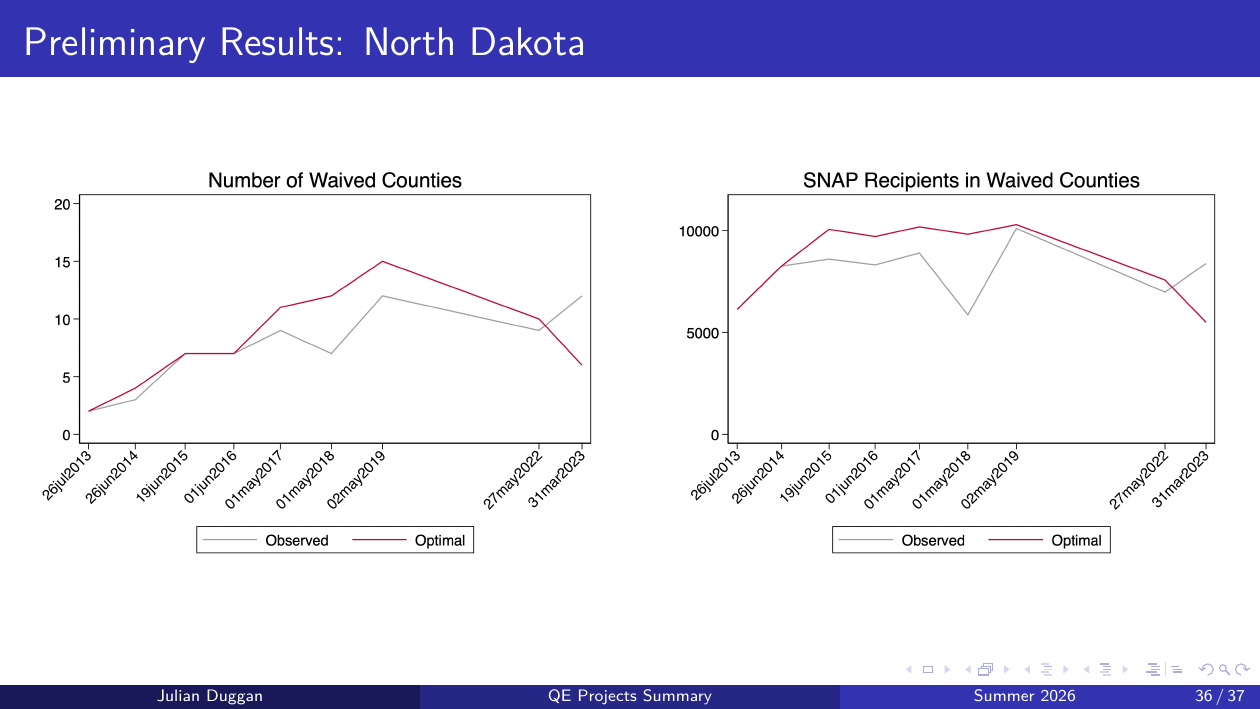
\includegraphics[width=0.6\textwidth]{duggan_nd_prelim}
% \end{center}
% \end{frame}

\end{document}
